\documentclass[../../../interview-questions.tex]{subfiles}

\begin{document}

\subsection{拦截器如何触发}

一直以为SpringMVC拦截器Interceptor是基于AOP实现的,然而事实并不是。 SpringMVC 中的Interceptor 拦截请求是通过HandlerInterceptor 来实现的。SpringMVC框架的核心类为DispatchServlet(org.springframework.web.servlet),http请求的核心执行方法doService(),我们画下SpringMVC的工作流程图:

\begin{figure}[htbp]
	\centering
	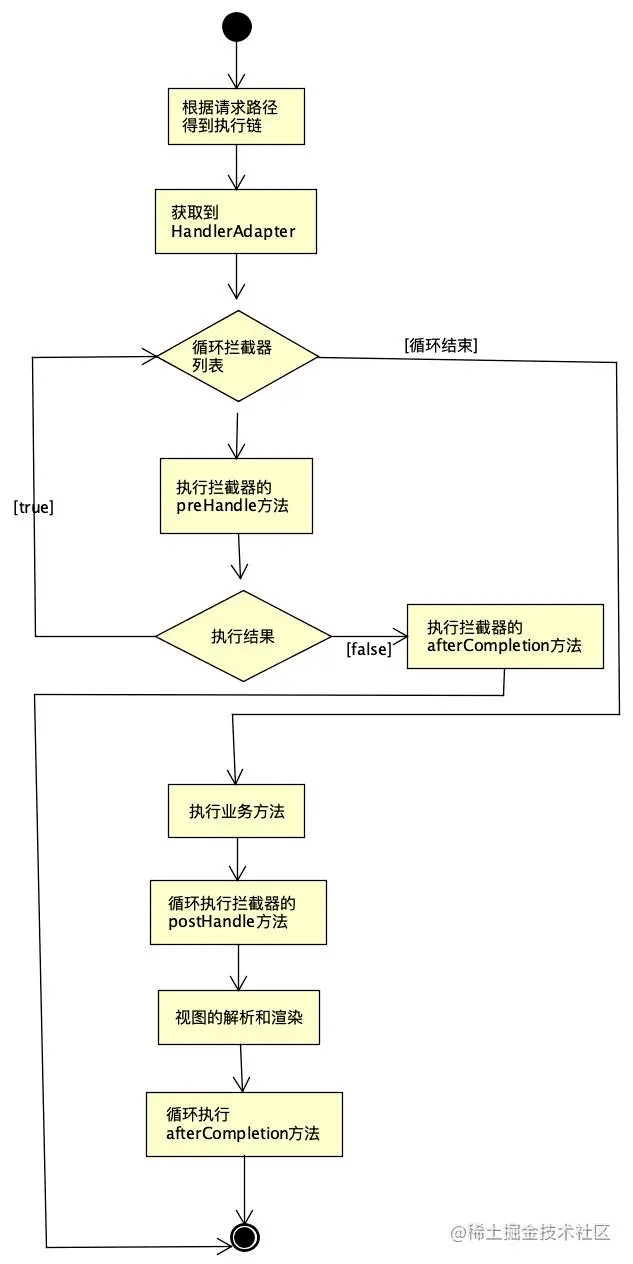
\includegraphics[scale=0.35]{interceptor.png}
	\caption{拦截器执行流程}
	\label{fig:interceptor}
\end{figure}

从流程图可以看到,拦截器的执行是在穿插在SpringMVC的工作流程中的,并没有用到动态代理机制,DispatchServlet的doDispatch方法直接调用的拦截器方法applyPreHandle和applyPostHandle。拦截器在实现层面,并没有用到AOP,并没有切面,通知这一类的代码,所以它的实现并不是基于AOP的。但是拦截器从思想层面上,是面向切面编程的,是在controller这个层面上进行的代码织入。HandlerInterceptor 接口中定义了三个方法,我们就是通过这三个方法来对用户的请求进行拦截处理的。

\begin{itemize}
	\item {preHandle (HttpServletRequest request, HttpServletResponse response, Object handle) 方法}
	\item {postHandle (HttpServletRequest request, HttpServletResponse response, Object handle, ModelAndView modelAndView) 方法}
	\item {afterCompletion(HttpServletRequest request, HttpServletResponse response, Object handle, Exception ex) }
\end{itemize}

\end{document}










